\section{Аналитическая часть}

\subsection{Составляющие компилятора}
Компилятор состоит из трёх частей.
\begin{enumerate}
	\item \textit{Frontend} преобразует текст программы на исходном языке во внутреннее представление, состоит из четырёх частей: препроцессор, лексический и синтаксический анализаторы, генератор внутреннего представления.  
	
	\item \textit{Middle-end} занимается машинно-независимой оптимизацией полученного внутреннего представления.
	
	\item \textit{Backend} выполняет преобразование внутреннего представления в программу на языке целевой платформы (ассемблер или машинный код).
\end{enumerate}

На рисунке \ref{fig:phases} изображены основные фазы работы компилятора.

\begin{figure}[h]
	\begin{center}
		{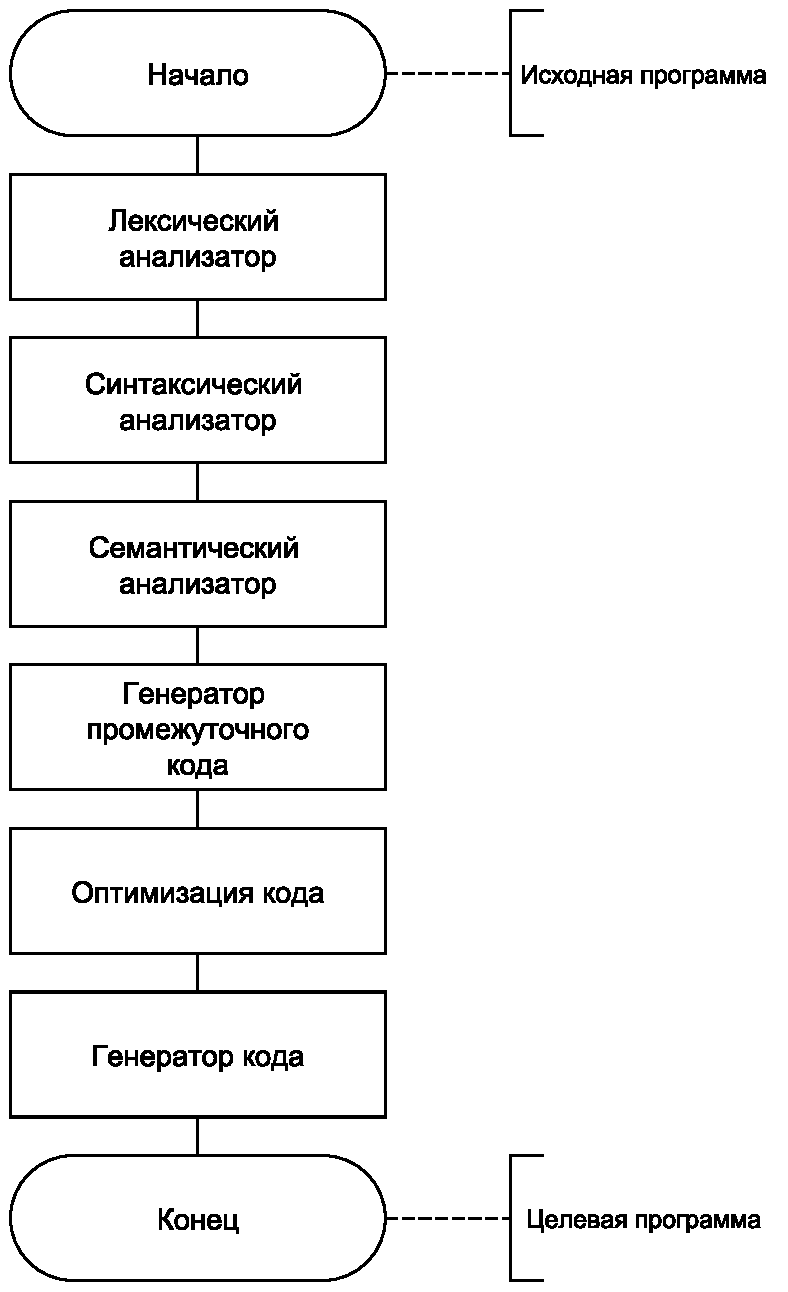
\includegraphics[scale = 0.53, page=1]{img/phases.pdf}}
		\caption{Фазы компилятора.}
		\label{fig:phases}
	\end{center}
\end{figure}

\subsection{Лексический анализатор}
Цель -- превратить поток символов в токены (этот процесс называется <<токенизацией>>). Выполняется группировка определённых терминальных символов в лексемы. Задаются конкретные правила в виде регулярных выражений, детерминированных конечных автоматов, грамматик. 

Лексический анализ может представляться как один из этапов синтаксического анализа. 

Обнаружение лексических ошибок, таких как недопустимые символы, ошибки идентификаторов или числовых констант, также является частью этого процесса. Кроме того, на этом этапе происходит удаление комментариев и обработка директив условной компиляции. \\

\subsection{Синтаксический анализатор}
Иерархический анализ называется разбором (<<parsing>>) или синтаксическим анализом, который включает группировку токенов исходной программы в грамматические фразы, используемые компилятором. Обычно они представляются в виде дерева. 

Обычно это представление выражается в виде абстрактного синтаксического дерева, где каждый внутренний узел является оператором, а дочерние -- его аргументами. Среди них можно выделить несколько групп связанных объектов:
\begin{itemize}
	\item элементы арифметических выражений: каждый узел представляет собой операцию и содержит её аргументы;
	
	\item элементы системы типов: базовые типы (числовые, строковые, структуры и т.п.), указатели, массивы и функции;
	 
	\item выражения пяти типов: арифметические, блочные и управляющие выражения, условные конструкции, циклы.
\end{itemize}

Разбор начинается со стартового нетерминала. 

Условные конструкции описывают конструкцию <<if>>, включающую в себя арифметическое выражение условия, выражение, выполняемое в случае его истинности, и альтернативное опциональное выражение.

Конструкции циклов (включают в себя <<while>>, <<do while>>, <<for>>) описывают арифметическое выражение условия и выражение, исполняемое в цикле.

Управляющие выражения -- <<break>>, <<continue>>, <<return>> и т.д. 

Блочные выражения -- последовательность других выражений, преимущественно используются в качестве тел функций и условных выражений и циклов.

Полученная грамматическая структура используется в последующих этапах компиляции для анализа исходной программы и генерации кода для целевой платформы. 

Синтаксический анализ выявляет синтаксические ошибки, относящиеся к нарушению структуры программы. \\

\subsection{Семантический анализатор}
В процессе семантического анализа проверяется наличие семантических ошибок в исходной программе и накапливается информация о типах для следующей стадии -- генерации кода. Используются иерархические структуры, полученные во время синтаксического анализа для идентификации операторов и операндов выражений и инструкций. 

Как правило, семантический анализатор разделяется на ряд более мелких, каждый из которых предназначен для конкретной конструкции. Соответствующий семантический анализатор вызывается синтаксическим анализатором как только он распознает синтаксическую единицу, требующую обработки.

Семантические анализаторы взаимодействуют между собой посредством информации, хранящейся в структурах данных, например, в центральной таблице символов. \\

\subsection{Генерация кода}
Последний этап -- генерация кода. Начинается тогда, когда во все системные таблицы занесена необходимая информация. В этом случае, компилятор переходит к построению соответствующей программы в машинном коде. Код генерируется при обходе дерева разбора, построенного на предыдущих этапах. 

Для получения машинного кода требуется два отдельных прохода:
\begin{itemize}
	\item генерация промежуточного кода;
	
	\item генерация собственно машинного кода.
\end{itemize}




\subsection*{Выводы}
Таким образом, в данной работе 
\pagebreak